\medskip

\begin{enumerate}
\item Ici, on interroge une personne au hasard, donc toutes les personnes qui constituent la population du pays ont la même probabilité d'être choisis : c'est une situation d'équiprobabilité et donc les proportions sont assimilables à des probabilités.

On a donc :
\begin{itemize}
\item $P(C) = 0,02$, car 2~\% de la population du pays a été contaminée;
\item $P(V) = 0,9$, car 90~\% de la population a été vaccinée;
\item $P_C(V) = 0,62$, car 62~\% des personnes contaminées ont été vaccinées.
\end{itemize}

\item 
	\begin{enumerate}
		\item On a :\quad $P(C \cap V) = P(C) \times P_C(V) = 0,02 \times 0,62 = 0,0124$.
		\item Les évènements $C$ et $\overline{C}$ partitionnent l'univers, donc, d'après la formule des probabilités totales :

$P(V) = P(C \cap V) + P\big(\,\overline{C}\cap V\big) \iff P\big(\,\overline{C} \cap V\big) = P(V) -
 P(C \cap V)$

On a donc : \quad $P\big(\,\overline{C} \cap V\big) = P(V) - P(C \cap V) = 0,9 - 0,0124 = \np{0,8876}$
	\end{enumerate}
\item Pour compléter l'arbre de probabilité, il nous faut $P_{\overline{C}}(V)$.

Par définition :\quad $P_{\overline{C}}(V) = \dfrac{P\big(\,\overline{C} \cap V\big)}{P\big(\,\overline{C}\,\big)} = \dfrac{0,8876}{1 - P(C)}=\dfrac{0,8876}{0,98} \approx 0,9057$ au dix-millième près.

Et donc : \hfill~
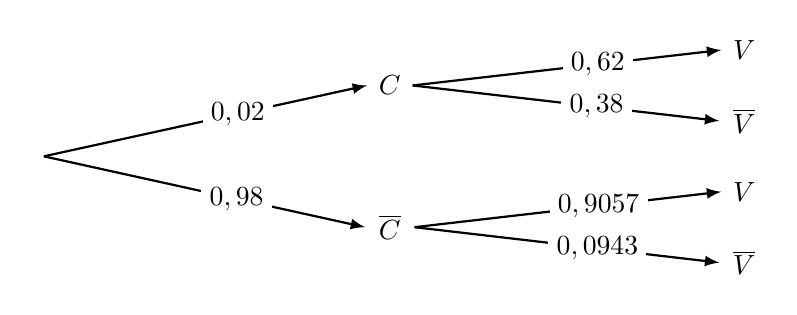
\begin{tikzpicture}[xscale=1,yscale=1,baseline={(R.base)}]

\tikzstyle{fleche}=[->,>=latex,thick]
\tikzstyle{noeud}=[fill=white,circle,inner sep=2pt]
\tikzstyle{feuille}=[fill=white,circle,inner sep=2pt]
\tikzstyle{etiquette}=[pos=0.6,fill=white, inner xsep=3pt, inner ysep=1.5pt]

\def\DistanceInterNiveaux{4.5}
\def\DistanceInterFeuilles{0.9}

\def\NiveauA{(0)*\DistanceInterNiveaux}
\def\NiveauB{(1)*\DistanceInterNiveaux}
\def\NiveauC{(2)*\DistanceInterNiveaux}
\def\InterFeuilles{(-1)*\DistanceInterFeuilles}

\node[noeud] (R) at ({\NiveauA},{(1.5)*\InterFeuilles}) {};
\node[noeud] (Ra) at ({\NiveauB},{(0.5)*\InterFeuilles}) {$C$};
\node[feuille] (Raa) at ({\NiveauC},{(0)*\InterFeuilles}) {$V$};
\node[feuille] (Rab) at ({\NiveauC},{(1)*\InterFeuilles}) {$\overline{V}$};
\node[noeud] (Rb) at ({\NiveauB},{(2.5)*\InterFeuilles}) {$\overline{C}$};
\node[feuille] (Rba) at ({\NiveauC},{(2)*\InterFeuilles}) {$V$};
\node[feuille] (Rbb) at ({\NiveauC},{(3)*\InterFeuilles}) {$\overline{V}$};

\draw[fleche] (R.east)--(Ra.west) node[etiquette] {$0,02$};
\draw[fleche] (Ra.east)--(Raa.west) node[etiquette] {$0,62$};
\draw[fleche] (Ra.east)--(Rab.west) node[etiquette] {$0,38$};
\draw[fleche] (R.east)--(Rb.west) node[etiquette] {$0,98$};
\draw[fleche] (Rb.east)--(Rba.west) node[etiquette] {$0,9057$};
\draw[fleche] (Rb.east)--(Rbb.west) node[etiquette] {$0,0943$};
\end{tikzpicture}
\hfill~

\item Par définition :\quad $P_V(C) = \dfrac{P(V \cap C)}{P(V)} = \dfrac{0,0124}{0,9} \approx 0,0138$.

Dans le contexte de l'exercice, cela signifie qu'environ 1,38~\% des personnes vaccinées ont été contaminées par le virus.

\item
	\begin{enumerate}
		\item \og Parmi les personnes non contaminées, il y a dix fois plus de personnes vaccinées que de personnes non vaccinées.\fg{}.

Cette affirmation est \textbf{fausse}, car un peu exagérée, parmi les personnes non contaminées, environ 90,57~\% d'entre elles sont vaccinées, quand 9,43~\% d'entre elles ne le sont pas, mais le décuple de 9,43~\% est 94,3~\%, qui est donc supérieur à 90,57~\%.

Il y a $\dfrac{90,57}{9,43}\approx 9,6$ fois plus de personnes vaccinées que non vaccinées parmi les personnes non contaminées.

		\item \og Plus de 98~\% de la population vaccinée n'a pas été contaminée.\fg{}

Cette affirmation est \textbf{vraie}, car on a calculé qu'environ 1,38~\% des personnes vaccinées ont été contaminées par le virus, donc, par complémentaire, cela implique qu'environ 98,62~\% des personnes vaccinées n'ont pas été contaminées. Il est donc correct de dire que c'est plus de 98~\%.
	\end{enumerate}
\item
	\begin{enumerate}
		\item 
\begin{itemize}
\item On a une épreuve aléatoire à deux issues. On qualifie de succès l'évènement $C$, de probabilité $p = 0,02$;
\item Cette épreuve est répétée $n =20$ fois pour constituer l'échantillon de 20 personnes. La répétition étant assimilable à des tirages successifs avec remise, on peut dire que les répétitions sont identiques et indépendantes;
\item La variable aléatoire $X$ compte le nombres de personnes contaminées, donc le nombre de succès, dans l'échantillon.
\end{itemize}

Ces trois éléments garantissent que $X$ suit la loi binomiale, de paramètres $n = 20$ et $p = 0,02$.

		\item La probabilité que 4 personnes exactement soient contaminées dans ce groupe de 20 personnes est :

			$P(X = 4) = \displaystyle \binom{20}{4}\times 0,02^4 \times 0,98^{20 - 4} = \np{4845}\times 0,02^4 \times 0,98^{16} \approx 5,6\times 10^{-4}$

Finalement, avec les consignes d'arrondi : \quad $P(X = 4) \approx 0,0006$
	\end{enumerate}
\end{enumerate}

\medskip
